

%\documentclass[12pt]{scrreprt}
\documentclass[12pt]{report} 

% language may be romanian or english (default is english)
% type may be bachelor or master (default is bachelor)
\usepackage[language=english, type=bachelor]{style}
\usepackage{graphicx}


\graphicspath{{./figures/}}

%\geometry{a4paper,top=2.5cm,left=3cm,right=2.5cm,bottom=2.5cm}
%in style
%controlling the appearance of your headers and footers
\usepackage{fancyhdr}
\pagestyle{fancy}
\lhead{}
\chead{}
\renewcommand{\headrulewidth}{0.2pt}
\renewcommand{\footrulewidth}{0.2pt}

\begin{document}

\specialization{German Informatics}	
\title{2FA Solidity Multisig Wallet}					   
\author{EȘAN TUDOR-CONSTANTIN}											
\supervisor{Grad, MIHAI-FLORIN-GABRIEL CRĂCIUN}				
				
\maketitle

\newpage
\thispagestyle{empty}
\mbox{}
\newpage
\pagenumbering{roman} 

\cleardoublepage
ABSTRACT
\vspace{0.5cm}	
\hrule
\vspace{0.5cm}	
%\cleardoublepage

\par Cryptocurrencies, digital assets for global money transfers, are reshaping how we think about finance. They use decentralized networks, allowing for faster, cheaper transactions without banks. Key benefits include almost instant payments, lower fees by eliminating middlemen, and the ability to transact worldwide.

\par The cryptocurrency journey began in the 1980s, revolutionizing in 2009 with Bitcoin's introduction by Satoshi Nakamoto. Bitcoin, leveraging blockchain technology, has become the best investment over the past decade, leading to widespread adoption and recognition, including the historic approval of the first Bitcoin ETF in January 2024. This not only showcases Bitcoin's status as a premier asset but also signals the mainstream financial world's embrace of cryptocurrencies.

\par Ethereum, introduced after Bitcoin, revolutionizes with smart contracts—automatic agreements executing conditions without human intervention. This technology enables decentralized applications (DApps) and decentralized finance (DeFi), transforming everything from voting systems to direct artist-to-fan sales without intermediaries.

\par However, operating without traditional banks isn't entirely without challenges. Cryptocurrency security hinges on private keys, unique digital signatures for accessing funds. For substantial sums, multisig wallets, requiring multiple approvals for transactions, become essential, providing an added layer of security against theft or unauthorized access, demonstrating the need for careful management in the expanding digital currency landscape.

\par Multisig, short for multi-signature, wallets offer enhanced security by necessitating approvals from multiple individuals before a transaction can proceed. This mechanism introduces an essential layer of collective decision-making, ensuring that funds cannot be moved at the whim of a single party. In this development, a novel addition is the integration of two-factor authentication (2FA) with the multisig process. This means that transactions require not just multiple approvals but also that one of these approvals must be verified through a separate 2FA process. This addition brings an extra layer of security to the transaction process, marrying the robustness of multisig protection with the familiar security feature of 2FA, a common safeguard in the wider digital banking and online services sphere, yet seldom applied in cryptocurrency transactions.

















\tableofcontents


\newpage
\pagenumbering{arabic}

\chapter{Introduction}


%\chapter*{Introduction}
\label{intro}

\section{Motivation}
\label{sec:ch1sec1}

\par Cryptocurrencies, digital assets for global money transfers, are reshaping how we think about finance. They use decentralized networks, allowing for faster, cheaper transactions without banks. Key benefits include almost instant payments, lower fees by eliminating middlemen, and the ability to transact worldwide.

\par The cryptocurrency journey began in the 1980s, revolutionizing in 2009 with Bitcoin's introduction by Satoshi Nakamoto. Bitcoin, leveraging blockchain technology, has become the best investment over the past decade, leading to widespread adoption and recognition, including the historic approval of the first Bitcoin ETF in January 2024. This not only showcases Bitcoin's status as a premier asset but also signals the mainstream financial world's embrace of cryptocurrencies.

\par Ethereum, introduced after Bitcoin, revolutionizes with smart contracts—automatic agreements executing conditions without human intervention. This technology enables decentralized applications (DApps) and decentralized finance (DeFi), transforming everything from voting systems to direct artist-to-fan sales without intermediaries.

\par Running a business without traditional banks is not without its difficulties, though. The secret digital signatures known as private keys are what make cryptocurrencies secure. The majority of users own non-custodial wallets, which give them complete control over their money and exclusive access to the private key. Although there are several advantages, there are also disadvantages. A person who loses their private key will no longer be able to access their entire fund, and since cryptocurrencies are decentralized, nobody can assist you. The fact that you won't be the only person with access to the money if your private key is taken and that you can't take back the money once it leaves your wallet is another issue, as discussed in the article by NEFTURE SECURITY \cite{Nefture2023Hack}
\begin{figure}[htbp]
	\centering
	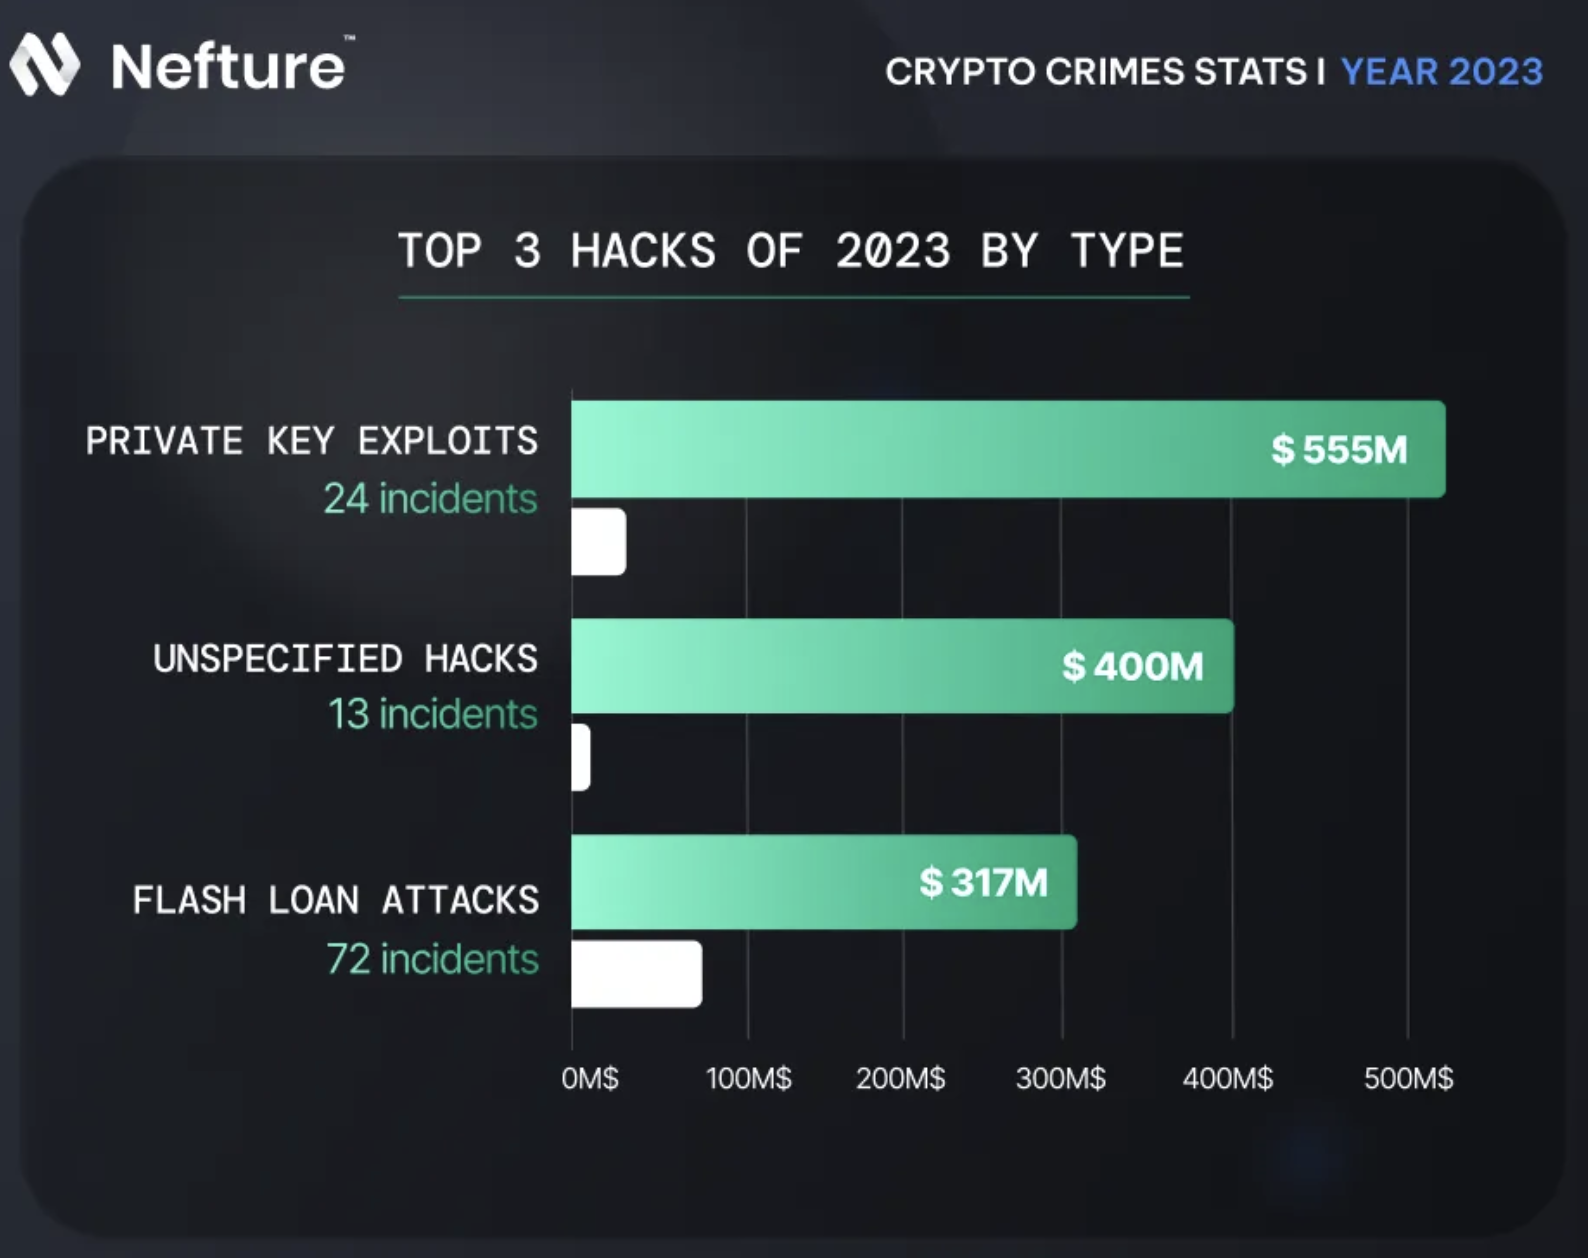
\includegraphics[scale=0.45]{./figures/stolen-pk.png}
	\caption{Total stolen funds value}
\end{figure}

\par A notable aspect that needs to be mentioned is that according to Nefture "Only 16.6\% of the contracts analyzed were managed by multisig wallets"\cite{Nefture2023Hack}. Using a multisig wallet can drastically reduce the probabilty of getting hacked especially if it was set up with multiple ownsers. This method lowers the possibility of unauthorized access to the system by requiring the consent of many parties prior to transactions being completed, adding an extra layer of security.


\section{Purpose}
\label{sec:ch1sec2}

\par The aim of this thesis is to develop a multisig wallet called "Vault" compatible with any EVM (Ethereum Virtual Machine) chain. Vault will provide a secure and efficient solution for managing digital assets across a wide range of blockchain platforms.
\par Vault will be a unified platform for managing digital assets across multiple EVM blockchains such as Ethereum, Base, Polygon etc. Users will be able to store, transfer and receive cryptocurrencies and NFTs easily and securely using a single interface. 
\par Vault is a simple to use multisig wallet that offers increased flexibility and security for managing digital assets. Unlike traditional wallets, Vault does not rely on a single private key, but uses a smart contract to distribute responsibility between multiple people or devices. This approach allows for personalized wallet configuration, perfectly adapting to individual needs and providing granular control over access to funds. Using smart contracts for this also allows for infinite configuration in the future. For features like: Key Recovery, Accounts Whitelisting (trusted accounts the wallet is allowed to interact with), Spending Limits, Subscriptions etc. 
\par Like any other multisig wallet the number of owners, and the approval threshold (the minimum number of signatures (approvals) execute a transaction) can be specified. This enables Vault to be used in a lot of different use cases:
\begin{itemize}
\item Shared Accounts: To enable cooperative fund management, several owners can be set up with a low approval requirement (for example, 1 of 2).
\item Enhanced Security: In order to guarantee access to funds even in the event of a lost private key, users can designate multiple private keys as owners. To improve security, a higher acceptance threshold (such as two out of three) might be specified.
\item Corporate Governance: The company's money can be transparently and democratically controlled by a board of directors acting as wallet owners, with a majority (i.e., 50\% + 1) vote required to approve transactions.
\end{itemize}

\section{Related work}
\label{sec:ch1sec3}

\par Multi-sig wallets offer a more secure solution for managing digital assets by sharing control between multiple people or devices. This section reviews relevant work related to multisig wallets, blockchain security protocols and multi-channel interoperability, contextualizing Vault in the existing landscape.
\par Currenlty some of the most used multisig wallets are:
\begin{itemize}
	\item Gnosis Safe: Since its 2018 launch, users have come to trust it because of its strong security and adaptable features. DApp integration: Allows for use in a variety of DeFi, NFT, and DAO scenarios by integrating with different DApp platforms. Smart contracts that have been audited: The wallet's smart contract code has been examined by recognized professionals, which lowers the possibility of security flaws. Decentralized governance: SafeDAO oversees the wallet's development, guaranteeing openness and participation from the community.
	\item Rabby Wallet: "Rabby Wallet is a Web3 wallet that offers a smooth multi-chain experience by automatically switching to the corresponding chain based on your visited Web3 dApp. Our security rule engine lets you check errors and risks before signing transactions. Rabby Wallet shows you the estimated balance change while you sign a transaction."\cite{rabbywallet}
	\item Argent X Wallet: "Argent is the first non-custodial wallet with no seed phrase and no complexity. With your Argent Vault, enjoy peace of mind through locking and unlocking your account, auto blocking transactions, and setting trusted contacts:"\cite{argent}
\end{itemize}

\par When compared to the other wallets, Vault's interface is far more straightforward and user-friendly. However, the Atlas 2FA feature is the best feature that no one else has. To put it simply, Vault allows you to set up a two-factor authentication code with Google authenticator. This code is required in addition to standard multisig security in order for the transaction to be completed. The best part is that you can configure your multisig to function as a wallet with one owner and one approval signature, but you can also turn on the Atlas for an additional security layer.
%\addcontentsline{toc}{chapter}{Introducere}
%\addcontentsline{toc}{chapter}{Introduction}

\chapter{Blockchain}

\section{Generalities}
\label{sec:ch2sec1}
A blockchain is a growing collection of items known as blocks that is stored in a decentralized, transparent, and secure ledger. Each block is linked to the previous one using hashes to form an unbreakable chain. Blockchains come are useful in a lot of scenarios where having a centralized middleman is not required. Currently, peer-to-peer currency represent the main use case for blockchain technology. cryptocurrencies that keep track of all user balances and transactions without the assistance of a single third. Bitcoin was the first blockchain of this kind as was defined as: "A purely peer-to-peer version of electronic cash would allow online payments to be sent directly from one party to another without going through a financial institution"\cite{nakamoto2008bitcoin}. The main characteristics of Bitcoin are:
\begin{itemize}
	\item Decentralisation: No sigle entity controlls the blockchain. It is managed by a distributed network of nodes.
	\item Imutability: Once a transaction is recorded on the blockchain it is almoast impossible to change it in the future
	\item Transparency: Everyone can view every transaction on the blockchain and everyones balance since the begining of the blockchain
	\item Security: Data on the blockchain is protected from modification and hacking by strong encryption.
\end{itemize}
\par With only 21 million bitcoins ever created, it is currently considered digital gold. Bitcoin was a groundbreaking idea. However, it is not without its shortcomings. Among them include the fact that Visa offers 24000 TPS whereas Bitcoin only allows 7 TPS (transactions per second). Another disadvantage is that fees are paid in Bitcoin. This meant that transactions were quite inexpensive when it initially launched, but since then, the price has increased from roughly zero to seventy thousand dollars, and fees have also increased. At the moment, a transfer costs about \$6, but this is becoming worse every day.
Because of this limitations since then over 1000 blockchains appeared according to Watcher Guru \cite{watcherguru}
\par Ethereum is the 2nd blockchain by market capitalization after bitcoin. After overcoming the early constraints of Bitcoin, the introduction of Ethereum signaled a turning point in the development of blockchain technology. Co-founder of Ethereum, Vitalik Buterin, pointed out that blockchain technology has applications beyond just transferring money. His goal was to build a programmable computer running code on top of Ethereum, a flexible framework for decentralised applications (DApps).
\par Buterin introduced the idea of a programmable blockchain with its own programming language, Solidity, for creating smart contracts in the Ethereum whitepaper, which was published in 2013. The description of Ethereum is "A Next-Generation Smart Contract and Decentralized Application Platform." \cite{ethereumwhitepaper}
\par The possibilities for blockchain are endless thanks to the capacity to write self-executing smart contracts. At its core, Ethereum is a worldwide network of nodes that can execute smart contract code thanks to the Ethereum Virtual Machine (EVM). Transaction fees or "gas" are paid for with ether money (ETH), which is also used to compensate network miners. Ethereum is now the foundation of a flourishing DApp ecosystem that is promoting innovation across many industries. The idea of Web3, which envisions a more user-based, decentralized internet, has been strengthened by it.

\section{Smart Contracts}
\label{sec:ch2sec2}
For a person that has not much experience with blockchain development, smart contracts are functions that are deployed on the blockchain and can be called by everyone. After the deployment the smart contract code cannot be altered. Investopidia defines smart contracts as: "a self-executing program that automates the actions required in an agreement or contract. Once completed, the transactions are trackable and irreversible. Smart contracts permit trusted transactions and agreements to be carried out among disparate, anonymous parties without the need for a central authority, legal system, or external enforcement mechanism"\cite{smartcontracts}. Some applications of smart contracts are the following:

Decentralized Finance (DeFi):
\begin{itemize}
	\item Liquid Staking: Users can stake their ETH on websites like as Lido or Rocket Pool, and in exchange, they will obtain liquid tokens equivalent to their ETH worth. Then, by using these liquid tokens in different DeFi protocols, more returns can be produced.
	\item Descentralized exchanges: Users can exchange various crypto-assets directly with one another without the necessity of centralized middlemen thanks to decentralized exchanges (DEX) like Uniswap and SushiSwap
	\item Lending and borrowing: Users can deposit or lend cryptocurrency assets to earn interest through platforms like Aave or Compound. All transactions are openly managed by smart contracts.
\end{itemize}

NFT Markets: Using smart contracts, marketplaces such as OpenSea or Rarible enable the buying, selling, and trade of unique tokens (NFTs), which stand in for digital art pieces, collectibles, or game assets.

 Decentralized autonomous organizations (DAO), such as MakerDAO, use smart contracts to enable token holders to speak up for themselves and cast votes on decisions that will determine the protocol's future development.
 
 Blockchain gaming: Smart contracts facilitate the management of game economies, include NFT components into the game, and guarantee a fair and transparent game for all players.
\chapter{Technologies}

\section{Solidity}
\label{sec:ch3sec1}
Solidity is a programming language that was created specifically for Ethereum smart contract creation \cite{sdocs} .The primary features are:

\begin{itemize}
	\item OOP: Solidity is an object-oriented programming language, which makes code organization and reuse simple. It is built on the idea of classes and objects.
	\item JavaScript-Like: Because of its core structure, which is similar to that of JavaScript, web professionals may easily learn Solidity. Its quirks have been tailored especially for blockchain, nevertheless.
	\item Solidity utilises static typing, which necessitates the specification of the data type of variables in advance. By doing this, compile-time errors are caught and contracts are enforced..
\end{itemize}

However given that smart contracts are deployed once and cannot be altered after you need to be very carefull about potential security risks that can lead to stolen funds. Some of the most common vulnerabilities are: Reentrancy Attacks, Integer Overflow/Underflow, Uninitialized Storage Pointers, Denial of Service (DoS) Attacks \cite{solidityVulnerabilities}

\section{Hardhat}
\label{sec:ch3sec2}
Hardhat is an open-source testing and development framework for Ethereum. The open-source framework for Ethereum development and testing \cite{hardhat}. It improves the process for creating and testing smart contracts. Hardhat is flexible; it supports numerous Solidity compilers and allows for different network configurations. Additionally, it may be expanded upon by combining it with additional blockchain ecosystem tools and frameworks. The comprehensive range of testing features contributes to the security and reliability of smart contracts. Hardhat strongly speeds up development, enhances the quality of the code, and lowers the possibility of mistakes in contracts that are well-written.

\section{Nextjs}
\label{sec:ch3sec3}
Next.js is an open-source React framework that extends the core React capabilities to create high-performance and SEO-friendly web applications. NextJs allows components to be rendered on the server, not only does it help with speed because the server can prerender the response but it can also help with webcrawlers to scan your site. The best features of NextJs include:
\begin{itemize}
	\item Image optimizations: "Automatically serve correctly sized images for each device, using modern image formats like WebP and AVIF." \cite{nextImage}
	\item Dynamic HTML Steaming
	\item Client And Server Components
	\item Server Actions: "Server Actions are asynchronous functions that are executed on the server. They can be used in Server and Client Components to handle form submissions and data mutations in Next.js applications." \cite{nextServerActions}
	\item Route Handlers: "allow you to create custom request handlers for a given route using the Web Request and Response APIs." \cite{nextRouteHandlers}
\end{itemize}

\section{Typescript}
\label{sec:ch3sec4}
"TypeScript adds additional syntax to JavaScript to support a tighter integration with your editor. Catch errors early in your editor"\cite{typescript}. Static types contribute to the reliability and maintainability of your code by reducing compilation errors. Classes make code more readable and scalable by enabling it to be divided into reusable modules. Compiling TypeScript into plain JavaScript makes it interoperable with every runtime and browser.
Using TypeScript has several advantages:
\begin{itemize}
\item Boost code quality: Static types make code more robust by assisting in the detection and prevention of compilation issues.
\item Boosts scalability: Code may be arranged into reusable modules by using classes and modules, which makes it simpler to create bigger projects.
\item Boost teamwork: Integrated documentation and static types can help enhance teamwork and communication.
\end{itemize}

\section{Tailwind}
\label{sec:ch3sec5}
Tailwind is defined as "a utility-first CSS framework packed with classes like flex, pt-4, text-center and rotate-90 that can be composed to build any design, directly in your markup" \cite{tailwind}.

Some of the Tailwind CSS's primary features are:
\begin{itemize}
\item Utility Classes: An extensive library of pre-made classes that style HTML components without requiring the creation of unique CSS code.
\item Components that can be customized: Enables the development of reusable parts with unique styles.
\item Expandable: Plugins can be added to expand the capabilities.
\end{itemize}
The Benefits of tailwind is that it drastically accelerates development, less CSS code writing is needed. There is no need in thinking what to name your css classes because they are pre defined. It minimizes the CSS file size, only the css needed is kept, the rest is "purged"

\section{RainbowKit}
\label{sec:ch3sec6}
RainbowKit is an open-source SDK that makes it it easier to incorporate Web3 wallets into your web apps. It gives consumers a range of alternatives by supporting multiple blockchains, including nearly every EVM compatible chain. RainbowKit's user-friendly interface lowers friction while facilitating a simple and seamless connection experience. Because of its customization capabilities, you can incorporate Web3 features unique to your project and alter the wallet's appearance. Rainbowkit also allows to easily change your chain whenever you like \cite{rainbowkit}

\section{Infura}
\label{sec:ch3sec7}
Infura is a platform that gives you access to blockchain nodes, drastically simplifying the process of connecting and interacting with blockchains such as Ethereum, IPFS, and Polygon, etc. By using Infura, you can save time and money by avoiding the hassle of configuring your own nodes. With the help of this platform's high scalability, security features, and quick access to blockchain data, you may create decentralized apps (dApps), incorporate blockchain technology into already-existing apps, and test concepts quickly without needing to design complicated infrastructure. \cite{infura}

\section{Etherscan}
\label{sec:ch3sec8}
The Etherscan API allows developers to access and query data from the Ethereum blockchain. It offers a wide range of functions that allow:
\begin{itemize}
	\item Get details about particular blocks, transactions, and accounts: You may find out information about balances, contract codes, and transaction histories for particular blocks, transactions, and accounts.
	\item Sending Transactions: You can call smart contract operations and transmit ETH transfers to the Ethereum network.
	\item Subscribe to events: You can get alerts in real time when new blocks or ETH transfers occur on the blockchain.
	\item Historical data query: The Ethereum blockchain provides historical information on blocks, transactions, and account statuses.\cite{etherscan}
\end{itemize}

\section{Viem}
\label{sec:ch3sec9}
Viem is a library that makes it easier and more natural for developers to work with the Ethereum network. Viem offers an abstraction over the implementation of the rpc methods used by EVM.\cite{viem}
Important aspects of Viem:
\begin{itemize}
\item Higher-level abstractions: Viem makes it simpler to work with notions like accounts, transactions, and smart contracts in your code by providing higher-level abstractions for them.
\item Defined Data Types: Viem increases the safety and readability of your code by predefining the data types that ethereum will use.
\item Multi-Chain Support: Polygon and Avalanche are two of the many Ethereum-compatible blockchains that Viem supports.
\item Simple integration: Viem interfaces with several well-known JavaScript frameworks and libraries with ease.
\end{itemize}

\section{Wagmi}
\label{sec:ch3sec10}
Wagmi is a library that greatly simplifies web3 development when utilizing React. To make communicating with the blockchain easier, Wagmi provides over 20 react hooks. These hooks can be used to get transactions, listen to events, or even communicate with other addresses or smart contracts. Additionally, Wagmi is the authorized connector for EIP-6963, walletconnect, and metamask. Tanstack useQuery enables Wagmi to assist with caching the get requests and avoiding deduplication. \cite{wagmi}

\section{useQuery}
\label{sec:ch3sec11}
useQuery is a library for the react framework that helps you with fetching data from external servers and doing mutations. It helps you with a lot of common task when dealing with this kind of use cases. This are some of its features
\begin{itemize}
	\item Prevents deduplication thanks to query keys
	\item Data Caching
	\item Error Handling
	\item Loading and Refetching handling
	\item Revalidating data after mutations
	\item Time based revalidation
\end{itemize}

\chapter{Vault Multisig Implementation}

\chapter{Conclusions}
%\chapter*{Conclusions}
\label{conclusions}
Significant improvements in the safety and flexibility of cryptocurrency transactions can be achieved using Vault, a powerful solution for controlling the security of digital assets and cryptocurrencies on the Ethereum chain.

By requiring many owners to approve transactions, multisig, or multiple signature, increases security by lowering the risks involved in managing a single access point. Even in the event that a private key is compromised, this approach restricts the likelihood of financial theft and prohibits unauthorized access.

The Atlas feature of the application is among its most inventive features. This feature adds an extra degree of protection and verification before transactions are finalized, much like the two-step authentication (2FA) systems seen in web-based apps. 

Because of its great versatility, the wallet may be configured in a variety of ways, from a single owner and approval level to simulating a 2FA wallet with Atlas capability. Users can adjust the security level to suit their own needs thanks to this. Additionally, money transfers require the 2FA code, even in the event that the single private key is compromised.

There are two primary areas that could be further addressed in terms of improvements. Since the contract already accepts ERC20 tokens, the first step would be to incorporate support for them directly into the application. By doing this, the wallet's functionality would be increased to support a larger variety of cryptocurrency assets. The second would be the development of a "Transaction Builder" page, such to what Safe provides \cite{transactionBuilder}, that would enable users to construct intricate transactions in a clear and simple manner, hence improving accessibility and transaction management efficiency.

In summary, Vault stands out for its successful synthesis of cutting-edge security, originality, and adaptability. It also has a great deal of room for future growth to better serve user demands.

%\addcontentsline{toc}{chapter}{Concluzii}
%\addcontentsline{toc}{chapter}{Conclusions}

\bibliography{references}

\end{document}
